\documentclass[12pt]{article}
\usepackage{ctex}
\usepackage{graphicx}  % 用于插入图片
\usepackage{amsmath}  % 数学公式支持
\usepackage{amssymb}  % 额外数学符号支持
\usepackage{listings}  % 用于插入代码
\usepackage{xcolor}  % 代码高亮
\usepackage{xcolor}    % 用于代码高亮
\usepackage{geometry}  % 用于设置页边距
\usepackage{subcaption}
\usepackage{booktabs}

\title{作业四~~样条插值法实验报告}
\author{姓名: 刘行~~学号: PB22000150}
\date{\today}
\begin{document}

\maketitle

\section{实验背景}
	样条插值是一种用于函数逼近的数值方法, 广泛应用于数据拟合、计算机图形学以及工程计算等领域. 本实验研究线性样条, 三次样条和 Hermite 样条的插值误差, 并分析其收敛阶.

\section{实验原理}
	样条插值的基本思想是使用分段低阶多项式函数来逼近给定的函数, 保证插值点处的函数值连续, 并在更高阶样条方法中保证导数的连续性.

\subsection{线性样条插值}
	线性样条插值使用线性函数在相邻的插值点之间进行插值, 其公式如下:
	\begin{equation}
		y = f(x_i) + \frac{f(x_{i+1}) - f(x_i)}{x_{i+1} - x_i} (x - x_i).
	\end{equation}

\subsection{自然三次样条插值}
	自然三次样条插值采用分段三次多项式逼近数据, 并通过构造合适的方程组保证函数值和导数的连续性,  以及区间边界处的二阶导为 $0$.

\subsection{Hermite 样条插值}
	Hermite 样条插值不仅使用函数值, 还利用导数信息进行插值, 其插值公式为:
	\begin{equation}
		y = h_{00}(t) f(x_i) + h_{10}(t) h f'(x_i) + h_{01}(t) f(x_{i+1}) + h_{11}(t) h f'(x_{i+1}),
	\end{equation}
	其中 $h_{00}$, $h_{10}$, $h_{01}$, $h_{11}$ 是 Hermite 基函数.

\section{代码思路}
	本实验使用 MATLAB 代码实现了不同方法的样条插值, 并计算了误差. 代码的主要流程如下:
	\begin{enumerate}
		\item 生成不同数量的节点.
		\item 计算不同插值方法的误差.
		\item 计算误差收敛阶.
		\item 绘制插值函数与真实函数的对比图.
	\end{enumerate}

\section{实验结果}
	实验输出了不同插值方法的误差及其收敛阶, 如下所示:
	\begin{verbatim}
		L1 error when interval_num = 3
		  1x1 struct
		     Linear: 0.0422
		      Cubic: 0.0161
		    Hermite: 0.0908
		L1 error when interval_num = 10
		  1x1 struct
		     Linear: 0.0412
		      Cubic: 0.0288
		    Hermite: 0.0013
		L1 error when interval_num = 20
		  1x1 struct
		     Linear: 0.0140
		      Cubic: 0.0064
		    Hermite: 1.8632e-04
		L1 error when interval_num = 40
		  1x1 struct
		     Linear: 0.0038
		      Cubic: 0.0015
		    Hermite: 1.4275e-05
		L1 error when interval_num = 160
		  1x1 struct
		     Linear: 2.4372e-04
		      Cubic: 8.9509e-05
		    Hermite: 5.9358e-08

		lin_ord
		  0.0240    1.6654    1.9515    2.0083
		cub_ord
		  -0.5716    2.3345    2.1900    2.0453
		her_ord
		  4.2369    2.9436    3.8397    4.0083
	\end{verbatim}

此外, 我们绘制了不同插值方法在 $3$ 段区间的情况下的拟合效果图, 如图 \ref{fig:interpolation} 所示.

\begin{figure}[ht]
	\centering
	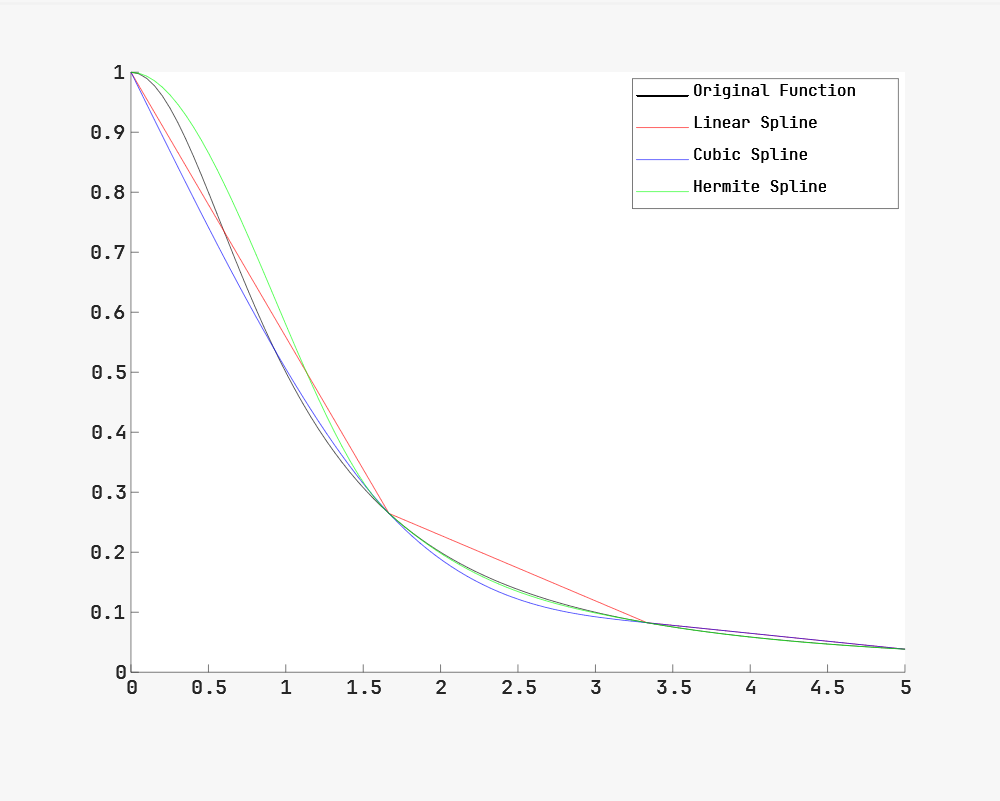
\includegraphics[width=0.8\textwidth]{figure/result.png}
	\caption{不同样条插值方法的插值结果}
	\label{fig:interpolation}
\end{figure}

\section{总结}
	实验结果表明:
	\begin{itemize}
		\item 线性样条插值的收敛阶为 $O(h^2)$.
		\item 三次样条插值的收敛阶为 $O(h^2)$.
		\item Hermite 样条插值的收敛阶为 $O(h^4)$.
	\end{itemize}
	实验结果符合理论预期, 说明 Hermite 样条插值方法在逼近精度上具有三者中最好的收敛性.

\end{document}
